%% It is just an empty TeX file.
%% Write your code here.

\documentclass[11pt]{article}
\usepackage[margin=1in]{geometry}
\usepackage{amsfonts, amsmath, amssymb}
\usepackage[none]{hyphenat}
\usepackage{fancyhdr}
\usepackage{graphicx}

\pagestyle{fancy}
\fancyhead{}
\fancyfoot{}
\fancyhead[L]{\slshape \MakeUppercase[Place Title Here]}

\DeclareMathOperator*{\argminA}{arg\,min} % Jan Hlavacek
\DeclareMathOperator*{\argminB}{argmin}   % Jan Hlavacek

\begin{document}

\section{Introdution}
As we know, people mostly get information and knowledge from news and articles. In this era, people are also used to using internet doing everything. So it’s no doubt that online news and articles are playing a very important role in our daily life. We can get any news we want through internet quickly. And also, it’s much easier to figure out which online news or articles we like through many internet ways, such like shares, likes and comments. \\ 
As we can imagine, popular news can make the authors become famous, also it can help the social media company attract more people. So they can make more profits. So if an author can know what can make news or articles become popular, or one company can predict whether news or articles will be popular before them are published, they will definitely try their best to get the information.  \\
So this project aims to find an method to predict how popular an online article can be before it is published by using several statistic characteristics summarized from it. We use the dataset from UCI Machine Learning Repository. In this dataset, it uses the number of shares for an online article to measure how popular it is.   

The input of algorithm is several features of Mashable articles: Words(e.g. number of words in the title), Links(e.g. number of Mashable article links), Digital Media(e.g. number of images), Time(e.g. day of the week), Keywords(e.g. number of keywords) and Natural Language Processing(e.g. closeness to top 5 LDA topics). We will predict the popularity in two perspectives. Firstly, we can use regression models(e.g. regression, GAM, Lasso) to predict the number of shares. Secondly, we make articles into 3 levels (unpopular, normal, popular) and then use classification algorithm(e.g. SVM, Random Forest, KNN) to find the articles level.  

\section{Method}
\subsection{Linear models}  
Linear models has been developed in age before computer came out, but we still study and use them a lot. If we have an input vector $X^T=(X_1,X_2,...,X_p)$, and want to predict a output Y. The linear regression model has the form $$Y=\beta_0+\sum_{j=1}^{p} X_j\beta_j$$
The linear model has one of assumptions. The regression function E(Y$\mid$X) is linear or it's reasonable to approximate it into linear model. In this formula, $\beta_j$s are unknown parameters, and variables $X_j$ can be in different sources.  
Also, there are seveal assumptions made for this model. We always assume that E(Y$\mid$X)=f(X) is a linear function of X and the error follows $\epsilon \sim \mathcal N(0, \sigma^2I)$ and $\epsilon$ uncorrelated with X and X is full rank which implies that X^T $\text{ is nonsingular and positive definite.}$

\subsection{Generalized Additive Models(GAM)}  
Linear models are good, but as the effects are often not linear in the real world, linear models often fail. We can use some more flexible statistical methods that can show nonlinear effects. We call these methods "generalized additive models". If we have an input vector $X^T=(X_1,X_2,...,X_p)$, and want to predict a output Y. The additive model has the form $$Y=\alpha+\sum_{j=1}^{p} f_j(X_j)+\epsilon$$
Where the mean of error term $\epsilon$ is 0. As each $f_j$ is an unspecified smooth nonparametric function. The approach is using an algorithm for simultaneously estimating all functions instead of expanding each function then fitted by simple least squares. Given observation $x_i$, $y_i$, the criterion is like: $$\sum_{i=1}^{N} (y_i-\alpha-\sum_{j=1}^{p}f_j(X_{ij}))^2+\sum_{j=1}^{p} \lambda_jf_j(X_{ij})$$

\subsection{Least Absolute Selection and Shrinkage Operator(lasso)}  
Lasso is another method for estimation in linear models. It solves the problem $$\min_{\beta} \sum_{i=1}^{n} (y_i-\sum_{j=1}^{p} x_{ij}\beta_{ij})^2 \text{, subject to } \sum_{j=1}^{p} \lvert \beta_j \rvert \leq t$$
Where t $\geq$ 0 is a parameter given by users. It controls the amount of shrinkage that is applied to the estimates. For the full least squares estimates $\hat{\beta}^0_j$, we can get $t_0=\sum_{j=1}^{p} \lvert \hat{\beta}^0_j \rvert$. $\forall t \leq t_0$ some $\beta_j$ will go to 0. We can also write as $$\hat\beta^{lasso}=\argminB_{\beta \in \mathbb{R}^p} \lVert y-X\beta\rVert^2_2+\lambda\lVert \beta \rVert_1$$
Where $\lambda=0$ gives ordinary least squares, $\lambda\to\infty$ gives $\hat\beta^{lasso}\to0$. 

\subsection{Support Vector Machines(SVM)}  
Besides the regression models, we can also classification algorithm to describe the result. Support Vector Machines are technique for constructing an optimal separating hyperplane between two classes. We can define SVM model as:$$\text{max }L(\alpha)=\sum_{i=1}^{n} \alpha_i - \frac{1}{2}\sum_{i=1}^{n}\sum_{i'=1}^{n}\alpha_i \alpha_i' y_i y_{i'} K(x_i,x_{i'})$$
    \begin{align}
        &s.t.  &0=\sum_{i=1}^{n} \alpha_iy_i \nonumber \\
        &      &0 \leq \alpha_i \leq C \nonumber
    \end{align}
Where the $K(x_i,x_{i'})$ is the kernel function. For this dateset, I try to use linear kernel and radial kernel.
    \begin{align}
        &\text{linear kernel}  &K(x_i,x_{i'})=<x_i,x_{i'}> \nonumber \\
        &\text{radial kernel}  &K(x_i,x_{i'})=exp(-\gamma \lVert x_i-x_{i'} \rVert^2) \nonumber
    \end{align}
For a multiclass classification, if we have K classes total, we can build K(K-1)/2 decision boundaries to decide one point should be put in which class.

\subsection{Random Forest} 
Random Forest is imporved from bagging. In bagging, we build a number of decision trees on bootstrapped training samples from the orginal dataset, and get the final prediction by using the most frequent class of all trees. But for growing the tree from the bootstrapped data, we select m variables at random from the p variables, instead of using all p variables to pick the best variables/split-point. With this idea, we can reduce the variance compared with bagging, by reducing the correlation between the trees.

\subsection{K-Nearest Neighbors(KNN)} 
This idea can be used both in regression and classification. The main thought is we try to estimate the result of x using the k points which are nearest to the x. For this dataset, we use Euclidean distance, and only use the most frequent class from k point to estimate the class of x.

\section{Data Analysis}
\subsection{Diagnostics}
For linear model: \\
    We don't choose a subset of feature to run the regression, as the dataset is not such large. From the fitted vs residual plot we can find that it goes well at the beginning, but as fitted value getting bigger the residuals become not so well. But we can still think the residuals are equally spreaded around a horizontal line without distinct patterns, so there is no non-linear relationships.   \\
    
    \begin{figure}[h]
        \centering
        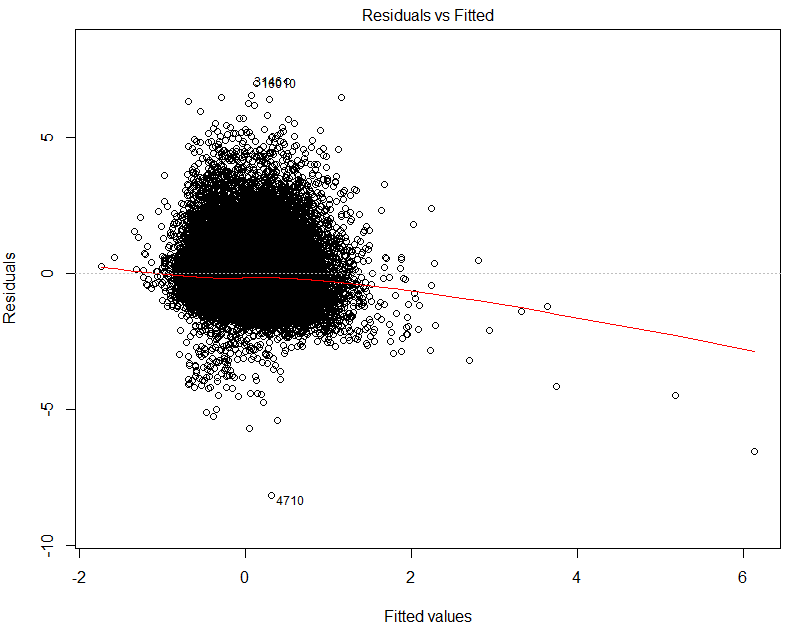
\includegraphics[width=0.7\linewidth]{linear_fvsr.png}
        \caption{Linear Regression Plot: Fitted vs Residuals}
    \end{figure}  
    
    As we look QQ plot, it shows that the residuals are not normally distributed so well. So we should have a concern about the residuals distribuion.\\
    
    \begin{figure}[h]
        \centering
        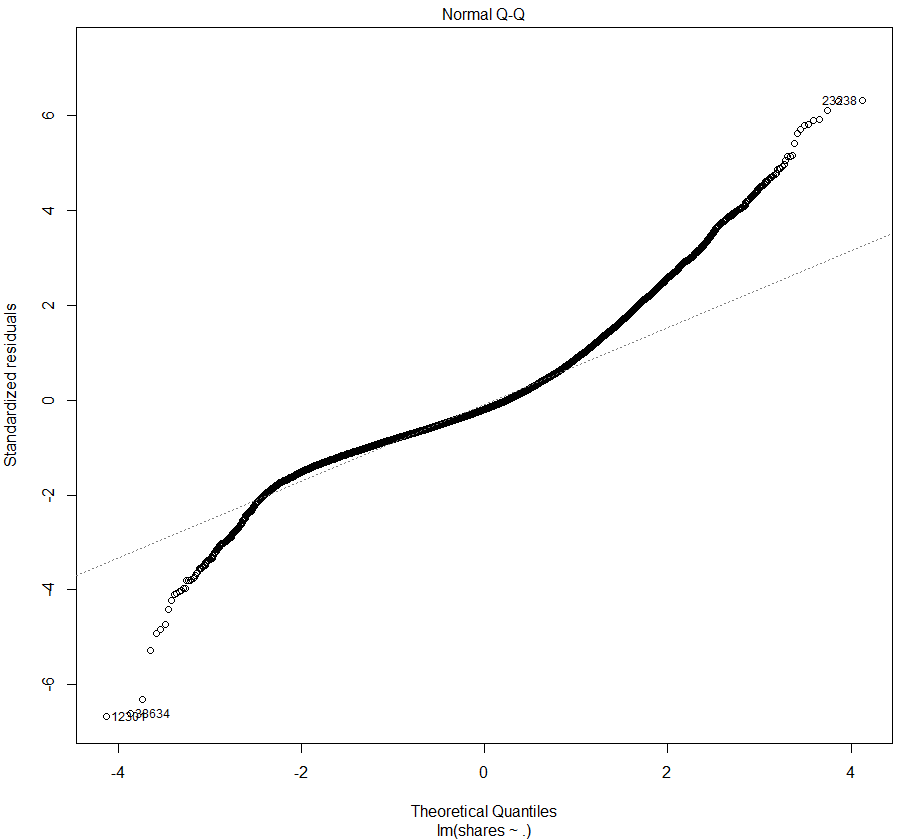
\includegraphics[width=0.7\linewidth]{linear_qq.png}
        \caption{Linear Regression Plot: QQ plot}
    \end{figure}    
    From the Scale-location plot, we can see the red line is continually going up, which suggests that the assumptions of equal variance of the residuals may not be true.  \\
    \begin{figure}[h]
        \centering
        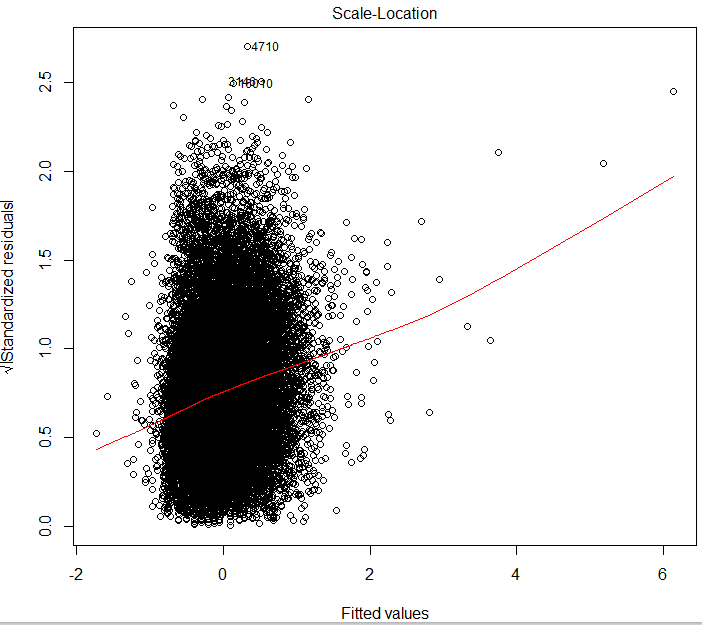
\includegraphics[width=0.7\linewidth]{linear_sl.png}
        \caption{Linear Regression Plot: Scale-location}
    \end{figure}
    
    For all variables, I calculate the vif for each of the variable, and some of their vif value are larger than 10, which shows the collinearity is significant in these variables. And we maybe can think about remove them. \\ 
For GAM: 
    From the method part, we know that $f_j(x_j)$ converges from $E \left[Y-\sum_{k \neq j}f_k(x_k)\mid{x_j} \right]$. We use gam model in R to fit the whole dataset, and according to model we get, we know that the number of local scoring iterations used to compute the estimates is only 9, which shows that this method converges pretty fast.
\subsection{Result}
\subsubsection{Regression}

\section{Conclusion}

\section{Appendix}

\end{document}